% ============================================================
%  深圳大学实验报告（SZU Experiment Report Template）
%  基于 Chao Fan / Kewei Ou 的模板修改
%  编译方式：Overleaf 选择 XeLaTeX
% ============================================================
\documentclass[a4paper,12pt]{article}

% ----------------------------
% 中文与字体支持
% ----------------------------
\usepackage{fontspec}
\usepackage{xeCJK}
\setCJKmainfont{Noto Serif CJK SC}

% ----------------------------
% 页面设置与常用宏包
% ----------------------------
\usepackage{geometry}
\geometry{left=1in, right=1in, top=1in, bottom=1in}

\usepackage{longtable}
\usepackage{graphicx}
\usepackage{fancyhdr}
\usepackage{tikz}
\usetikzlibrary{calc}
\usepackage{float}
\usepackage{xcolor}
\usepackage{booktabs}
\usepackage{amsmath}
\usepackage{amssymb}
\usepackage{array}
\usepackage{listings}
\usepackage{url}
\usepackage[hidelinks]{hyperref}

% 本报告用红色标出本人实现的部分
\newcommand{\mine}[1]{\textcolor{red!85!black}{\textbf{#1}}}

\lstset{
  basicstyle=\ttfamily\scriptsize,
  breaklines=true,
  columns=fullflexible,
  frame=single,
  rulecolor=\color{gray!45},
  backgroundcolor=\color{gray!6},
  escapeinside={(*@}{@*)},
  showstringspaces=false,
  aboveskip=4pt,
  belowskip=4pt,
  xleftmargin=2pt,
  xrightmargin=2pt
}

\fancyhf{}
\fancyhead[C]{}

% ============================================================
\begin{document}

% ============================================================
% 封面
% ============================================================
\begin{titlepage}
    \centering
    \vspace*{1.6cm}
    \Huge{\textbf{深 \ 圳 \ 大 \ 学 \ 实 \ 验 \ 报 \ 告}}\\[1.3cm]

    {\Large\textbf{课程名称}\quad\underline{\makebox[8cm][c]{Python 程序设计}}}\\[0.45cm]
    {\Large
    \noindent\makebox[3.2cm][l]{\textbf{项目名称}}
    \underline{\makebox[8cm][c]{\footnotesize Project 1：ViT-B/32 图像编码器}}}\\[0.45cm]
    {\Large
    \noindent\makebox[3.2cm][l]{\textbf{学 \quad \quad 院}}
    \underline{\makebox[8cm][c]{人工智能学院}}}\\[0.45cm]
    {\Large
    \noindent\makebox[3.2cm][l]{\textbf{专 \quad \quad 业}}
    \underline{\makebox[8cm][c]{}}}\\[0.45cm]
    {\Large
    \noindent\makebox[3.2cm][l]{\textbf{指导教师}}
    \underline{\makebox[8cm][c]{舒婷}}}\\[0.45cm]
    {\Large
    \noindent\makebox[3.2cm][l]{\textbf{报 \quad 告 \quad 人}}
    \underline{\makebox[3cm][c]{}}
    \hspace{0.4cm}
    \textbf{学号}
    \underline{\makebox[3cm][c]{}}}\\[0.45cm]
    {\Large
    \noindent\makebox[3.2cm][l]{\textbf{实验时间}}
    \underline{\makebox[8cm][c]{}}}\\[0.45cm]
    {\Large
    \noindent\makebox[3.2cm][l]{\textbf{提交时间}}
    \underline{\makebox[8cm][c]{}}}\\[1.2cm]

    \vfill
    \Large{\textbf{教务处制}}
\end{titlepage}

\newpage

% ============================================================
% 正文
% ============================================================
\section{Objectives}

本项目的目标是在\textbf{不依赖 PyTorch 与 OpenCLIP} 的条件下，仅用 NumPy
复现 OpenCLIP ViT-B/32 图像塔的前向计算。输入是经过 shortest-edge
resize、center crop 和均值/方差归一化后的 $B\times3\times224\times224$
浮点图像；输出是每张图一个 $B\times512$ 的单位向量。模型固定为
12 层、宽度 768、12 个注意力头、patch 大小 32，共 152 个视觉张量，
全部由课程提供。因此本实验只涉及前向数值计算，不涉及任何训练或参数更新。

\section{Overview}

整体数据流如图~\ref{fig:pipeline} 所示。图像被切成 $7\times7$ 个
$32\times32$ 的 patch，每个 patch 按 $C,H,W$ 展平成 3072 维，得到
$49\times3072$ 的 patch 矩阵；经无 bias 的线性投影变为 $49\times768$，
在 token 0 拼接一个 CLS 行并加上 $50\times768$ 的位置编码；随后依次通过
12 个结构相同的 Transformer block；最后只取 CLS 行，做 LayerNorm、
$768\to512$ 投影和 L2 归一化，得到输出 token。

\begin{figure}[H]
    \centering
    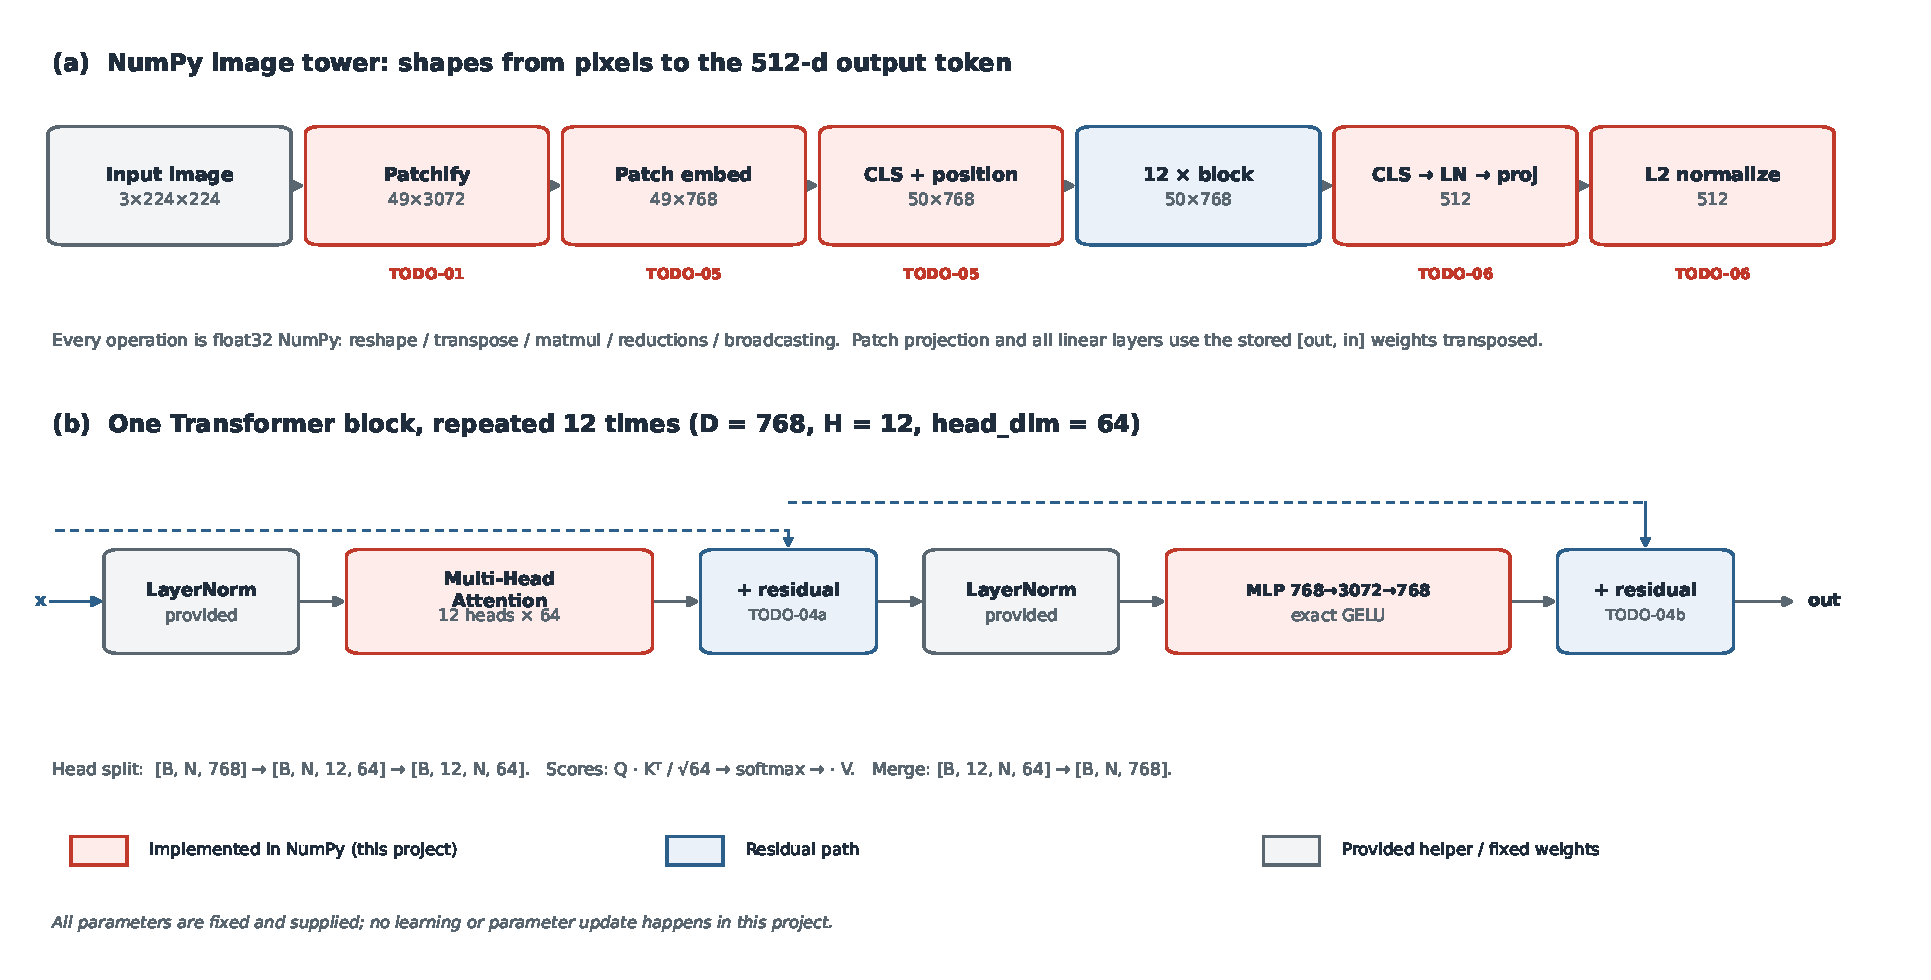
\includegraphics[width=\linewidth]{figs/pipeline.pdf}
    \caption{OpenCLIP ViT-B/32 图像塔的数据流与单层结构。\mine{红色}为本人用
    NumPy 实现的部分（TODO-01$\sim$06），蓝色为残差路径，灰色为课程提供的
    helper 与固定权重。}
    \label{fig:pipeline}
\end{figure}

实现严格遵循 checkpoint 的约定：patch 投影和所有线性层按 $[out,in]$ 存储，
计算时乘权重转置；只有 \texttt{visual.proj} 是 $[in,out]=[768,512]$，直接右乘；
LayerNorm 的 $\epsilon=10^{-5}$；激活函数使用与权重匹配的精确
$\mathrm{GELU}(x)=0.5x\left(1+\mathrm{erf}(x/\sqrt2)\right)$。所有中间数组
保持 \texttt{float32}。

\section{Implementations}

本人只修改 \texttt{image\_encoder.py}，下面按数据流顺序说明六个 TODO 的
实现。代码中的红色行是本人补充的核心语句。

\subsection{Patch 划分与嵌入（TODO-01、TODO-05）}

直接对 $[B,3,224,224]$ 做一次 \texttt{reshape(B,49,3072)} 会把通道与空间
位置交错，patch 顺序就错了。正确做法是先拆出 patch 网格的两个轴，再重排：

\begin{lstlisting}[language=Python]
def patchify(self, images):
    b, c, h, w = images.shape                 # 224, 224
    grid = images.reshape(b, c, h//32, 32, w//32, 32)
    (*@\textcolor{red!85!black}{\textbf{grid = grid.transpose(0, 2, 4, 1, 3, 5)}}@*)
    return np.ascontiguousarray(grid).reshape(b, 49, 3072)
\end{lstlisting}

形状变化为
$[B,3,224,224]\to[B,3,7,32,7,32]\to[B,7,7,3,32,32]\to[B,49,3072]$，
其中 transpose 的后三个轴恰好是 $C,H,W$，保证展平顺序与参考一致。
嵌入阶段用 \texttt{patches @ patch\_weight.T}（无 bias）得到 $[B,49,768]$，
再用 \texttt{np.concatenate} 把 CLS 放在 token 0，最后与 $[50,768]$ 的
位置表相加，广播到整个 batch。

\subsection{多头注意力（TODO-02、TODO-03）}

\texttt{split\_heads} 把特征轴拆成 12 组、每组 64 维：
$[B,N,768]\to[B,N,12,64]\to[B,12,N,64]$。注意力计算为

\begin{equation}
Q=XW_q^{\top}+b_q,\quad K=XW_k^{\top}+b_k,\quad V=XW_v^{\top}+b_v,
\end{equation}
\begin{equation}
S=\frac{QK^{\top}}{\sqrt{64}},\qquad
A=\operatorname{softmax}(S),\qquad
C=AV .
\end{equation}

其中 $Q,K,V\in\mathbb{R}^{B\times12\times N\times64}$，$S,A\in\mathbb{R}^{B\times12\times N\times N}$。
这里 $K$ 是 4 维张量，只能交换最后两个轴（\texttt{k.transpose(0,1,3,2)}），
不能写成二维的 \texttt{k.T}，否则会把 batch 和 head 也交换。得到
$C$ 后，先用 \texttt{transpose(0,2,1,3)} 还原成 $[B,N,12,64]$，再
\texttt{reshape} 成 $[B,N,768]$ 合并多头，最后做输出投影
$C W_o^{\top}+b_o$。

\subsection{Transformer block（TODO-04）}

每个 block 有两条残差：

\begin{align}
R &= X + \operatorname{MHA}(\operatorname{LN}_1(X)),\\
Y &= R + \operatorname{MLP}(\operatorname{LN}_2(R)),
\end{align}

其中 $\operatorname{MLP}(u)=\mathrm{GELU}(uW_1^{\top}+b_1)W_2^{\top}+b_2$，
中间维度为 3072。两条残差都加在\textbf{未归一化}的输入上；若把
$\operatorname{LN}_1(X)$ 当作残差起点，误差会迅速放大。该 block 没有
LayerScale 参数，这点也与 checkpoint 一致。

\subsection{输出 token（TODO-06）}

12 层之后得到 $[B,50,768]$，只取第 0 行：
\begin{equation}
z=\operatorname{LN}_{post}\!\left(T[:,0]\right),\qquad
\hat z=\frac{z\,W_{proj}}{\lVert z\,W_{proj}\rVert_2},
\end{equation}
其中 $W_{proj}$ 直接右乘、不再转置。最终 $\hat z\in\mathbb{R}^{B\times512}$，
每行长度为 1。

\section{Results}

实验环境为 Python 3.14.6、NumPy 2.4.6、Pillow 12.3.0，普通 CPU，无 GPU。
运行 \texttt{python check.py --stage all} 的逐级结果如表~\ref{tab:errors}，
其中参考值由独立的 Torch FP32 前向和最终项目的教师参考给出。输出阶段的
容差为 $\mathrm{atol}=2\times10^{-5}$、$\mathrm{rtol}=2\times10^{-4}$；
内部 token 为 $\mathrm{atol}=2\times10^{-4}$。

\begin{table}[H]
\centering
\small
\renewcommand{\arraystretch}{1.12}
\begin{tabular}{lccrrl}
\toprule
Stage & Shape & max$|\Delta|$ & mean$|\Delta|$ & 结果 \\
\midrule
preprocess  & $(10,3,224,224)$ & $0$            & $0$            & PASS \\
patches     & $(2,49,3072)$    & $0$            & $0$            & PASS \\
tokens      & $(2,50,768)$     & $4.58\times10^{-5}$ & $1.31\times10^{-6}$ & PASS \\
block0      & $(2,50,768)$     & $6.35\times10^{-6}$ & $3.28\times10^{-7}$ & PASS \\
last\_tokens& $(2,50,768)$     & $4.86\times10^{-5}$ & $2.74\times10^{-6}$ & PASS \\
output      & $(10,512)$       & $4.92\times10^{-7}$ & $8.00\times10^{-8}$ & PASS \\
batch       & $(3,512)$        & $4.25\times10^{-7}$ & $7.78\times10^{-8}$ & PASS \\
\bottomrule
\end{tabular}
\caption{逐级数值检查结果（全部通过）。}
\label{tab:errors}
\end{table}

\texttt{batch} 一项把图片顺序改成 $[1,0,1]$（含重复）后重新计算，误差仍在
容差内，说明实现没有按位置缓存参考结果。10 张图的完整前向约 6.07 秒，
\texttt{run.py} 输出的 \texttt{output\_tokens.npz} 形状为 $(10,512)$，
每行 L2 范数为 $1.000000$。

\section{Discussion}

\paragraph{一个 shape 变化。}
patchify 是本项目里形状变化最剧烈的一步：输入
$[B,3,224,224]$，输出 $[B,49,3072]$。关键是先拆成 6 维
$[B,3,7,32,7,32]$，把 patch 行列 $(7,7)$ 移到通道前面，再按
$(C,32,32)$ 展平。若省略这一步、直接 reshape，虽然形状仍是
$(B,49,3072)$，但每个 patch 内部混入了不同通道和不同空间位置的像素，
后续所有层都会在错误的 token 上计算。

\paragraph{一个修掉的 bug。}
最初我确实用了 ``直接 reshape'' 的写法：
\texttt{images.reshape(B,49,3072)}。\texttt{patches} 检查立即失败，
最大绝对误差为 $3.938$、平均绝对误差为 $0.986$，远超
$2\times10^{-4}$ 的容差，但形状完全正确，很容易误判。改为上面的
6 维 reshape + \texttt{transpose(0,2,4,1,3,5)} 后，patches 的误差降为
$0$，后续 tokens、block0 也依次通过。这个 bug 说明：\textbf{形状对不等于
语义对}，调试时应先看中间数组的数值，而不是只看 shape。

\paragraph{局限与改进。}
当前实现是纯 NumPy、单线程 CPU，10 张图约 6 秒，其中 \texttt{helpers.GELU}
用逐标量 \texttt{math.erf} 实现，是主要瓶颈。浮点误差主要来自矩阵乘法的
累加顺序，输出最大误差 $4.9\times10^{-7}$，余量充足。该编码器可直接作为
最终项目 \texttt{szu\_python\_openclip} 的图像塔，与文本塔组合做图文检索；
但本项目的 152 个张量只是视觉部分，不能替代最终项目的完整多模态
checkpoint。

\paragraph{贡献与协助。}
本人完成了 \texttt{image\_encoder.py} 中六个 TODO 的 NumPy 实现、
12 道 NumPy 练习、逐级数值调试与报告撰写；课程提供了模型权重、
\texttt{helpers.py}、\texttt{check.py} 及参考输出。开发过程中使用了
AI 编程助手辅助整理思路、检查 shape 与润色文字，所有结论和数值均在
本地运行 \texttt{check.py} 复现。代码仓库：
\url{https://github.com/xizixuan0103/project1-numpy-encoder}。

\newpage

% ============================================================
% 批阅与成绩评定页
% ============================================================
\begin{tikzpicture}[remember picture, overlay]
  \draw[thick]
    ($(current page.north west)+(2cm,-3cm)$)
    rectangle
    ($(current page.south east)+(-2cm,3.5cm)$);
\end{tikzpicture}

\vspace{1cm}

\noindent \textbf{指导教师批阅意见：}
\vspace{6cm}
\hfill

\vspace{1cm}

\noindent \textbf{成绩评定：}
\vspace{2cm}
\hfill

\vspace{1cm}

\noindent
\hfill
\textbf{指导教师签字：}\quad\quad\quad\quad\quad\\[0.5cm]

\hfill
\textbf{年}\quad\quad
\textbf{月}\quad\quad
\textbf{日}\quad

\vspace{1cm}

\noindent \textbf{备注：}

\begin{tikzpicture}[remember picture, overlay]
  \node[
    anchor=north west,
    inner sep=0pt,
    text width=\dimexpr\paperwidth-4cm\relax
  ] at ($(current page.south west)+(2cm,3.1cm)$) {
    \begin{minipage}{\dimexpr\paperwidth-4cm\relax}
      \small
      \noindent
      \textbf{注：}\;1、报告内的项目或内容设置，可根据实际情况加以调整和补充。\\[0.2cm]
      \phantom{\textbf{注：}\;}2、教师批改学生实验报告时间应在学生提交实验报告时间后 10 日内。
    \end{minipage}
  };
\end{tikzpicture}

\end{document}




